\begin{surferPage}[216 Singularities]{Plohe s puno realnih singulariteta}
		Kao \v sto smo ve\' c spomenuli, to\v can najve\' ci mogu\' ci broj singulariteta $\mu(7)$ 
		na plohi stupnja $7$ jo\v s uvijek nije poznat. Poznata nam je samo donja i 
		gornja granica za taj broj: $99\le \mu(7) \le 104$.
		
		
		Dakle, nije iznena\dj uju\' ce to \v sto op\' cenito o plohama stupnja $d$ znamo jo\v s i manje.
		
		Sonja Breske, Oliver Labs i Duco van Straten su uspjeli prilagoditi 
		konstrukciju od S.V.\ Chmutova tako da trenutni maksimalan broj singulariteta 
		dose\v zu i plohe s realnim singularitetima.
		Ono \v sto dosada znamo je sljede\' ce:
		\[0,41\bar{6}d^3 \lessapprox \mu(d) \lessapprox 0.44\bar{4} d^3.\]
		Ako gledamo odozgo, mogu\' ce je uo\v citi simetri\v cnost konstrukcije, kao i 
		poveznicu s maksimalnim brojem crnih \' celija u razmje\v staju pravaca:
		\begin{center}
      \begin{tabular}{c@{\qquad}c}
        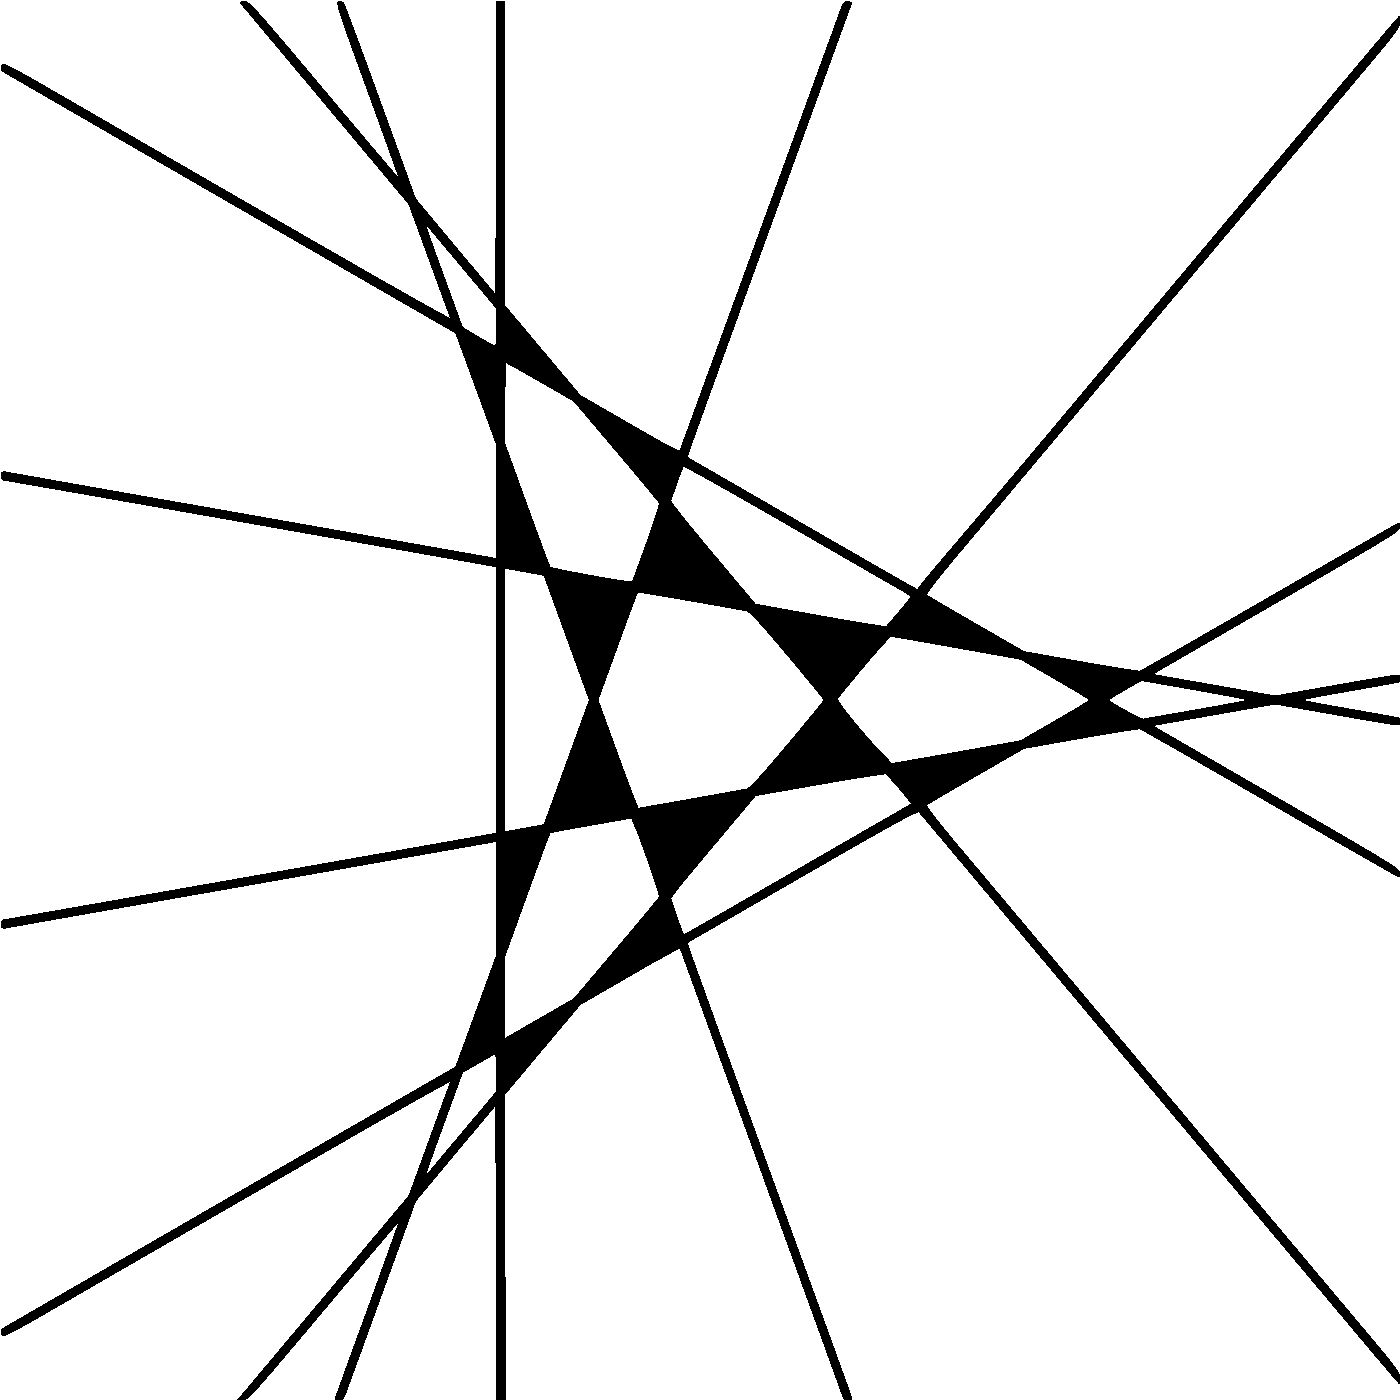
\includegraphics[height=1.5cm]{./../../common/images/vielesing.pdf}
        &
        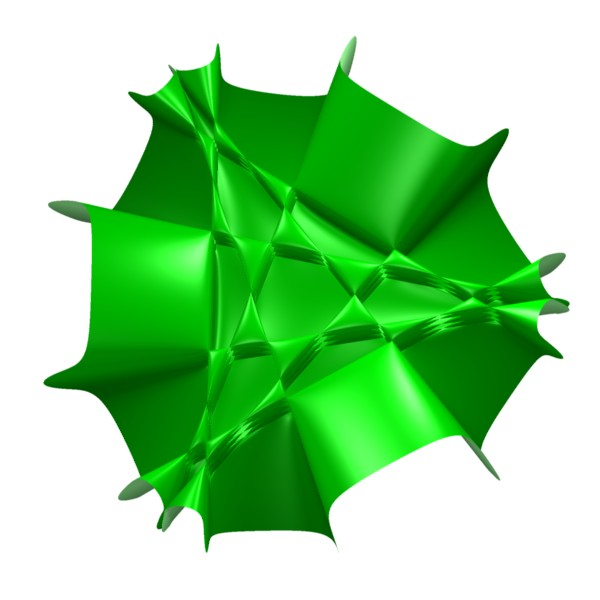
\includegraphics[height=1.5cm]{./../../common/images/p9surface_von_oben}
      \end{tabular}
    \end{center}
\end{surferPage}
